\chapter{DTLS: tinydtls} \label{Chp: DTLS}

DTLS is the another widely considered security measure in the WSN community. Comparing to Link Layer security measures such as 802.15.4 Security, DTLS is implemented at a higher level and thus is more flexible. 

On Contiki, DTLS is provided by a third party module tinydtls. The current version of tinydtls supports only two ciphersuites, namely TLS\_PSK\_WITH\_AES\_128\_CCM\_8 \\
and TLS\_ECDHE\_ECDSA\_WITH\_AES\_128\_CCM\_8. Since both ciphersuites use AES-128 CCM for data encryption and are only different during handshake; hence we do not distinguish them when analysing the application data\cite{TlsRenego}.

The data in this chapter are all collected for CC2538.

\section{Protocol and Implementation}

Due to the fact that tinydlts implements only minimum features of DTLS, we have found most attacks in \cite{rfc7457} not applicable in this scenario. To be more specifically,

\begin{itemize}
	\item WSN devices tend to support only minimum, usually only single, protocols due to constrained resources; thus downgrade attacks are unlikely to be a threat.
	\item The block cipher is used in CTR mode and thus immune to Padding Oracle Attacks.
	\item RC4 is excluded by DTLS; therefore its attacks are also excluded.
	\item No compression is implemented and thus Compression Attacks are also excluded.
	\item RSA is not used in the ciphersuites and its attacks are thus excluded.
	\item tinydtls is hardcoded to support only secp256r1 curve, thus is immune to Diffie-Hellman Parameters attacks.
\end{itemize}

Exceptionally, Renegotiation vulnerability\cite{rfc5746} may exist in the tinydtls implementation as the counter measure, Renegotiation Indication Extension, is not supported in tinydtls. This vulnerability allows a man-in-the-middle adversary to inject data into the DTLS session. In case of web applications, for example, this allows the adversary to inject malicious code into a HTTP request sent by the client\cite{TlsRenego}.

\section{DTLS Handshake}

\textbf{[To be done...]}

\section{Data Size}

The exact size of data in DTLS Data Records are directly visible in the captured packets, as highlighted in the middle of \Cref{Fig: Size of application data in a DTLS Data Record}.

\begin{figure}[ht!]
	\center
	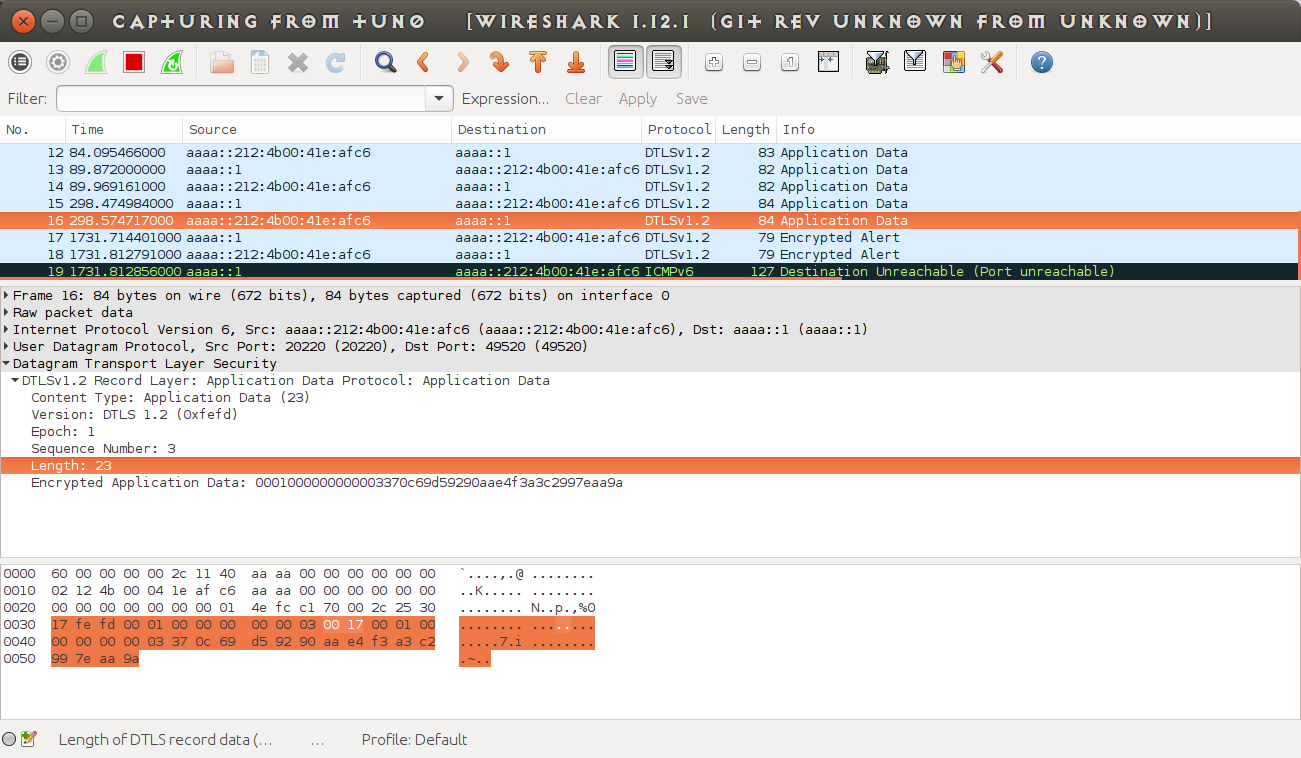
\includegraphics[width=.9\linewidth]{fig/dtlslength.png}
	\caption{Size of application data in a DTLS Data Record}
	\label{Fig: Size of application data in a DTLS Data Record}
\end{figure}

The size of application data is exactly the value of highlighted Length field in the middle of \Cref{Fig: Size of application data in a DTLS Data Record} minus $16$ bytes, as explained in \cite{rfc5116}.

%Practically length is useful ,but we don't go further.%
In practice data length is one of the most widely exploited side channel information in Traffic Analysis attacks, but it is also highly dependent to the upper layer application. Without loss of generality, we leave the analysis of data length to specific applications.

\section{Packet Timing}

The second column in \Cref{Fig: Size of application data in a DTLS Data Record} is the timing of packets being sent. In this section, we analyse the timing feature of applications protected by tinydtls on Contiki.

\subsection{Processing Model}

\Cref{Fig: A Session with DTLS} illustrates the procedure of a Session protected by DTLS. For example, packet No.15 and No.16 in \Cref{Fig: Size of application data in a DTLS Data Record} are a Session of two Sensor Nodes exchanging application data, where No.15 is the Request and No.16 the Response. 

\begin{figure*}[ht!]
	\center
	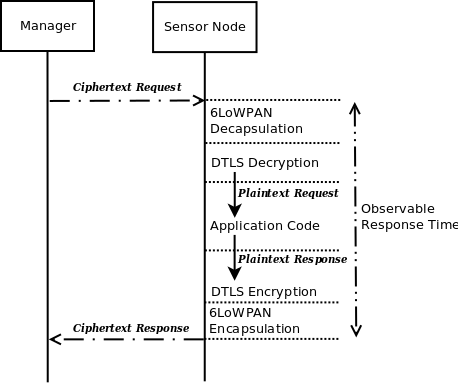
\includegraphics[width=0.8\textwidth]{fig/dtls_session.png}
	\caption{A Session with DTLS}
	\label{Fig: A Session with DTLS}
\end{figure*}

The observable response time is calculated as the time difference of Request and Response in the captured traffic, e.g. the response time of pakcet No. 15 and No.16 in \Cref{Fig: Size of application data in a DTLS Data Record} is $298.574717 - 298.474984 = 0.099733 \text{(s)} = 99.733 \text{(ms)}$. From a practical aspect, we consider the accuracy of measurement to be $10^{-4}$ s ($10^{-1}$ ms).

DTLS provides protections between only two Sensor Nodes in the network; thus the source and destination are consistent within the a DTLS session. The 6LoWPAN encapsulation and decapsulation procedure are identical for all packets within the same DTLS session as the headers are basically identical except the sequence numbers. We therefore consider 6LowPAN decapsulation and encapsulation takes a constant time.

The observable response time in \Cref{Fig: A Session with DTLS} can be divided into two parts:
\begin{enumerate}
	\item Protocol suite processing time. This part consists of the 6LoWPAN decapsulation / encapsulation and DTLS decryption / encryption. We assume the code of this part is independent to the application code and is identical among all applications.
	\item Application code execution time. It is one of the most interested information to adversaries that could be exploited to learn information about the application data.
\end{enumerate}

For simplicity, we denote $t_R$, $t_P$ and $t_A$ to be the observable response time, protocol suite processing time and application code execution time respectively. Apparently we have:
\begin{equation}
t_R = t_P + t_A
\end{equation}

Therefore a method to extract $t_A$ is to compute it by 
\begin{equation} \label{Eq: t_A}
t_A = t_R - t_P
\end{equation}

From an information leakage aspect,$t_A$ may be exploited to correlate the data in the packet. In later this section, we focus on how it can be approximated from $t_R$, which is directly accessible in the captured traffic.

\subsection{AES Timing} \label{tinydtls AES Timing}

tinydtls uses the OpenBSD optimised AES implementation. Its source code is available at:\\ 
\url{https://github.com/Salties/MyRepository/blob/master/tinydtls-0.8.2/aes/rijndael.c}

We applied the same tests as described in \Cref{Sec: AES Timing}. The average AES execution time is shown in \Cref{Tbl: tinydtls AES execution time estimation} and the Fixed vs Random test is shown in \Cref{Tbl: Fixed vs Random test result for tinydtls AES execution time on CC2538}.

\begin{table}[ht!]
	\center
	\begin{tabular}{|c|c|}
		\hline
		                        & CC2538 SW \\ \hline
		50 executions           & 160.07          \\ \hline
		100 executions          & 320.06          \\ \hline
		150 executions          & 480.05          \\ \hline
		200 executions          & 640.13          \\ \hline
		Ticks per executions    & 3.20            \\ \hline
		AES Execution Time (ms) & 0.098           \\ \hline
	\end{tabular}
	\caption{tinydtls AES execution time estimation}
	\label{Tbl: tinydtls AES execution time estimation}
\end{table}

\begin{table}[ht!]
	\center
	\begin{tabular}{|c|c|c|}
		\hline
		                         & Fixed       & Random      \\ \hline
		Sample Mean              & 640.28      & 640.25      \\ \hline
		Sample Standard Deviation & 0.49        & 0.53        \\ \hline
		t-score                  & \multicolumn{2}{c|}{1.32} \\ \hline
	\end{tabular}
	\caption{Fixed vs Random test result for tinydtls optimised AES execution time on CC2538. Executions per sample: $200$. Sample size: $1000$, measured in ticks.}
	\label{Tbl: Fixed vs Random test result for tinydtls AES execution time on CC2538}
\end{table}

Applying the TVLA t-score threshold $4.5$, the result in \Cref{Tbl: Fixed vs Random test result for tinydtls AES execution time on CC2538} concludes that the optimised AES implementation has passed our test, i.e. no leakage is detected through the execution time. 

The result is consistent with our expectation, as the implementation has no branch\footnote{The only branch in the source code is for AES-192 and AES-256, which are not used in the ciphersuites.} in the source code and is done with only statements of assignment, shift and XORs. The low sample standard deviation is also an evidence that supports our expectation that the AES implementation takes a nearly constant time. We conclude that the timing difference of $t_P$ induced by AES execution is negligible.

The source code and data for our tinydtls AES timing experiments are available at: \\
\url{https://github.com/Salties/MyRepository/tree/master/experiments/dtlsaes} \\
and \\
\url{https://github.com/Salties/MyRepository/tree/master/experiments/dtlsaes/Data}

\subsection{Protocol Suite Processing Timing} \label{Protocol Suite Processing Time}

Theoretically, given a specific platform the value of $t_P$ is predictable, as it is independent to the upper layer application and the choice of different DTLS session keys does not affect the timing as shown in \Cref{tinydtls AES Timing}. We therefore assumed it is identical among all applications and estimated it on CC2538 by an application where the Sensor Node replies to any Requests with a constant predefined value. Our source code is illustrated in \Cref{nullapp}.

\lstinputlisting[label={nullapp}, captionpos=b, caption={Application code with negligible execution time}]{src/nullapp.c} 

Since no effective application code exists in this application, its $t_A$ can be considered negligible; hence $t_R$ can be viewed as an approximation of $t_P$:
\begin{equation}
t_R = t_P + t_A \approx t_P + 0 = t_P
\end{equation}

Avoid exceeding 802.15.4 MTU, the length of DTLS Payload ranges from $1$ byte to $46$ bytes in general. However in our setup the Response is sent in an one hop transmission and hence its TTL in IPv6 Header is compressed, allowing the Response for one extra byte.

\Cref{Fig: Example histograms of protocol suite processing time on CC2538 with DTLS} shows two example histograms of part of our result. We denote $|Req| \in [1,46]$ and $|Res| \in [1,47]$ as the length in bytes of the DTLS Payload in Requests and Responses respectively.

\begin{figure}[ht!]
	\center
	\begin{subfigure}{.8\textwidth}
	\center
	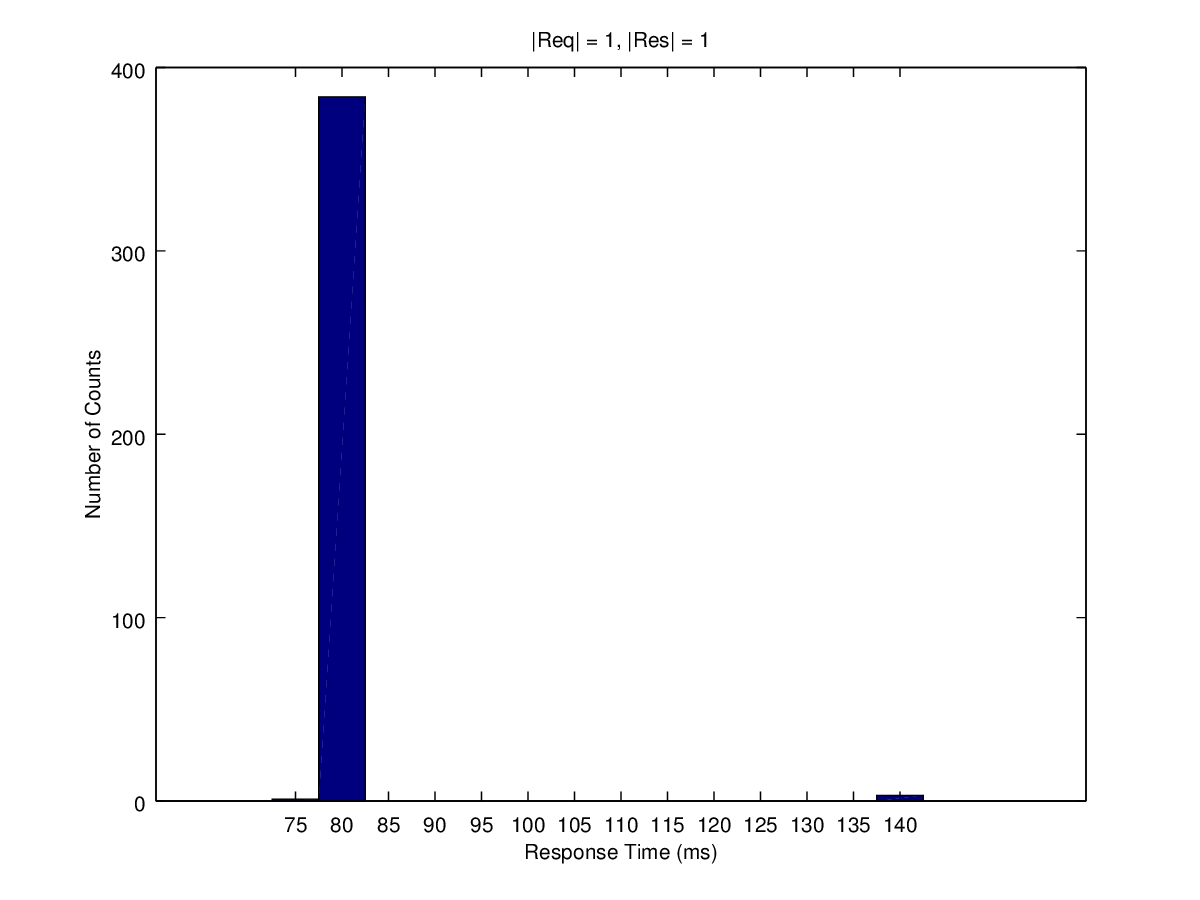
\includegraphics[width=\linewidth]{fig/dtlstimehist_min.png}
	\end{subfigure}
	\begin{subfigure}{.8\textwidth}
	\center
	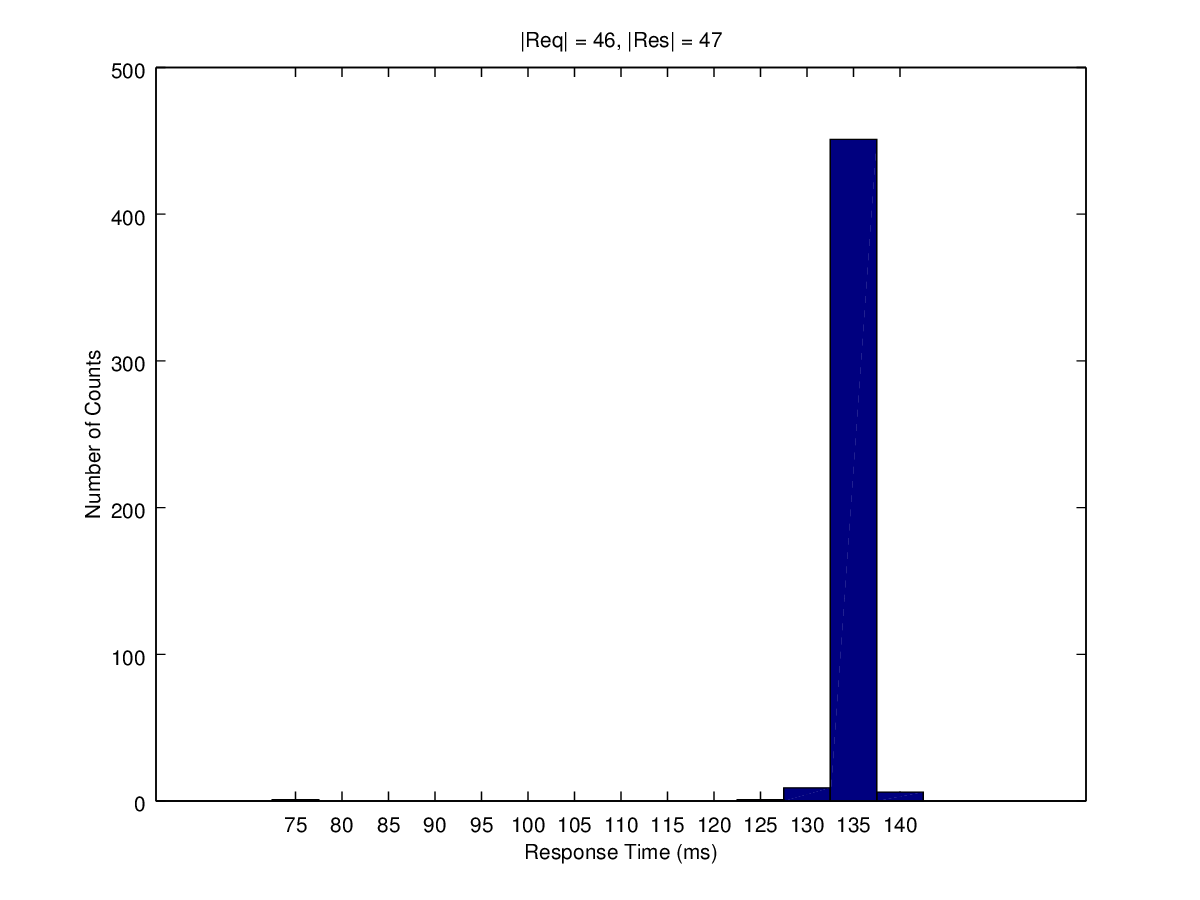
\includegraphics[width=\linewidth]{fig/dtlstimehist_max.png}
	\end{subfigure}
	\caption{Example histograms of protocol suite processing time on CC2538 with tinydtls}
	\label{Fig: Example histograms of protocol suite processing time on CC2538 with DTLS}
\end{figure}

Similar to the ECHO response time,$t_R$ in the samples also appeared to densely clustered near a specific value with a few outliers; hence we use the sample median to characterise $t_R$ in our experiments. Medians of the examples in \Cref{Fig: Example histograms of protocol suite processing time on CC2538 with DTLS} are summarised in \Cref{Tbl: Median of response times in examples}. The data shows that when $|Req|$ and $|Res|$ are at their maximum value, $t_R$ is significantly longer comparing to $Req$ and $Res$ at their minimum value.
 
\begin{table}
	\center
	\begin{tabular}{|c|c|c|}
		\hline
		 				&($|Req| = 1$, $|Res| = 1$) 	& ($|Req| = 46$, $|Res| = 47$) 	\\ \hline
		 Sample Median	&79.712 ms                  			& 132.740 ms                   			\\ \hline
	\end{tabular}

	\caption{Medians of response time in the examples of \Cref{Fig: Example histograms of protocol suite processing time on CC2538 with DTLS}}
	\label{Tbl: Median of response times in examples}
\end{table}

\Cref{Fig: Protocol suite processing time on CC2538 with DTLS} shows $t_R$ with different combinations of $|Req|$ and $|Res|$.

\begin{figure}[ht!]
	\center
	\begin{subfigure}{0.8\linewidth}
	\center
	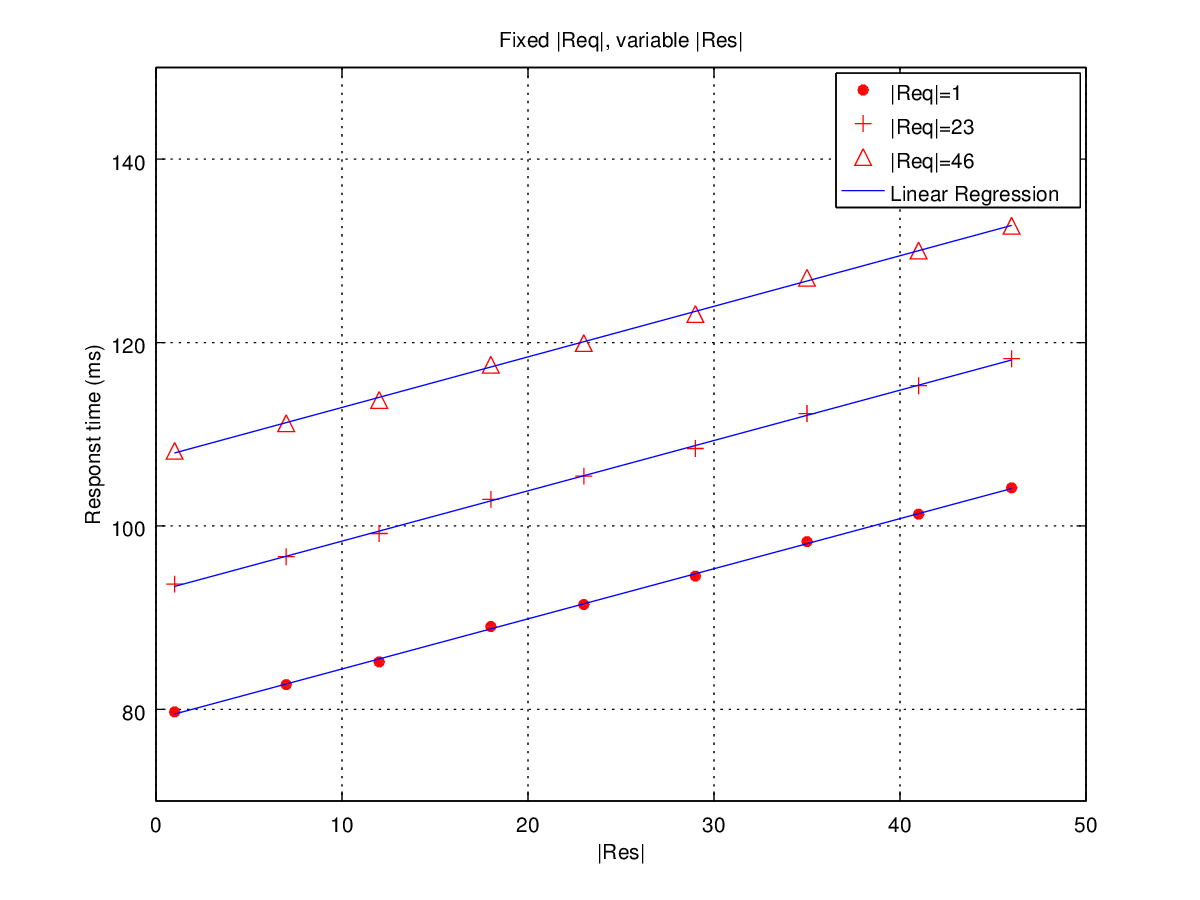
\includegraphics[width=\textwidth]{fig/dtlstime_fixed_req.png}
	\subcaption{Response time($t_R$) with $|Req| \in \{1, 23, 46\}$}
	\end{subfigure}
	\begin{subfigure}{0.8\linewidth}
	\center
	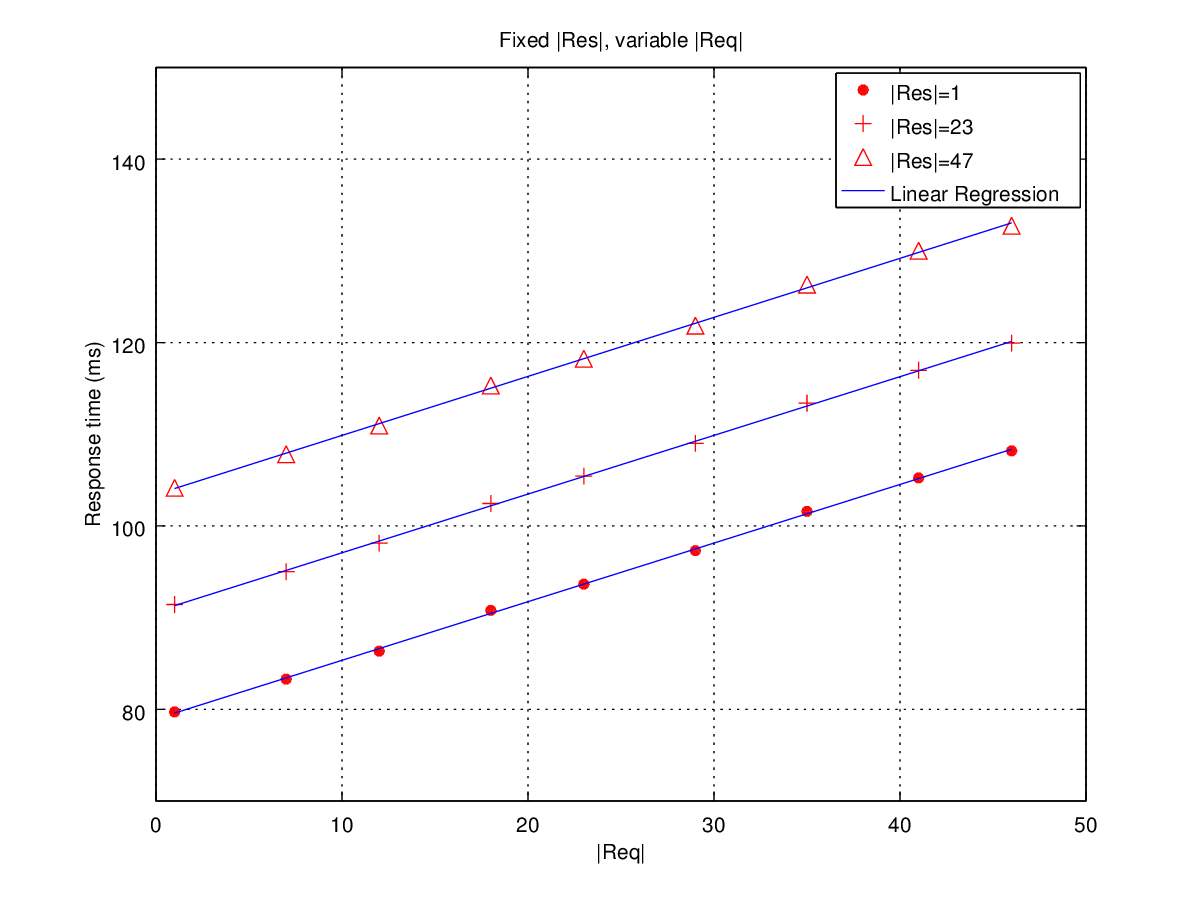
\includegraphics[width=\textwidth]{fig/dtlstime_fixed_res.png}
	\subcaption{Response time($t_R$) with $|Res| \in \{1, 23, 46\}$}
	\end{subfigure}
	\caption{Protocol suite processing time on CC2538 with DTLS}
	\label{Fig: Protocol suite processing time on CC2538 with DTLS}
\end{figure}

\Cref{Fig: Protocol suite processing time on CC2538 with DTLS} suggests that $|Req|$ and $|Res|$ might be multi linear to $t_R$. Therefore we assume $t_R$ is in the form of:
\begin{equation} \label{Eq: tR est}
	t_R = b_0 + b_1|Req| + b_2|Res|
\end{equation}

Applying multiple linear regression using least squares fit, we have an estimation of $t_R$ (in ms), denotes as $\hat{t}$, for CC2538:
\begin{equation}
	\hat{t}_R = 78.388 + 0.538|Req| + 0.638|Res|
	\label{Eq: t_R estimation}
\end{equation}

The $R^2$ for the extimation of \Cref{Eq: t_R estimation} is $0.9997$ with $F=87778$ ($F_{0.05} = 3.18$). The result indicates that $t_R$ is significantly linearly related to $|Req|$ and $|Res|$.

Since $t_A$ in this application (\Cref{nullapp}) is negligible, we therefore approximate $t_P$ by $t_R$:
\begin{equation} \label{Eq: CC2538tP}
	\hat{t}_P \approx \hat{t}_R = 78.388 + 0.538|Req| + 0.638|Res|
\end{equation}

\Cref{Eq: CC2538tP} is our estimation of the protocol suite processing time for a CC2538 Sensor Node using Contiki release-3.0 with tinydtls, upon observing a Request of length $|Req|$ with Response of length $|Res|$.

In practice, assume the adversary has the pre-knowledge of the type of device, he can profile and estimate $t_P$ as we have done on CC2538. Given the estimation $\hat{t}_P$, we can further estimate the the application execution time by substituting $t_P$ in \Cref{Eq: t_A} by $\hat{t}_P$:
\begin{equation} \label{Eq: hattA}
	\hat{t}_A = t_R - \hat{t}_P
\end{equation}
where $t_R$ is directly accessible in the captured traffic. We discuss more details of the estimation of \Cref{Eq: hattA} in \Cref{App code timing}.

The source code and data for our protocol suite processing timing experiments are available at: \\
\url{https://github.com/Salties/MyRepository/tree/master/experiments/dtlstime} \\
and \\
\url{https://github.com/Salties/MyRepository/tree/master/experiments/dtlstime/Data}

\subsection{Application Code Timing} \label{App code timing}

\Cref{Eq: hattA} provides a method to estimate the application code execution time on a Sensor  Node. To test this method, we used an application that repeatedly invokes the Contiki system random number generator according to the data in the Request, and replies the execution time as the Response. The random number generator is selected arbitrary simply for a controllable $t_A$. In real world applications, the loop is replaced by actual application code, such as reading a sensor, data processing, or any application over CoAP, etc. The code of this application is illustrated by \Cref{apptime}.

\lstinputlisting[label={apptime}, captionpos=b, caption={Code for application code timing}]{src/dtlsapptime.c} 

We tested \Cref{Eq: hattA} of application in \Cref{apptime} on CC2538, with different execution time and arbitrary length of data, using $t_P$ estimated by \Cref{Eq: CC2538tP}. The actual execution time of $t_A$ is obtained by the execution time sent in Response.

We also denote their absolute and relative approximation error as $\epsilon$ and $\mu$ respectively, where:
\begin{eqnarray}
	\begin{aligned}
		\epsilon	&= |t_A - \hat{t}_A| \\
		\mu 	&= \epsilon / |t_A|
	\end{aligned}
\end{eqnarray}

For clarity of the view of data, we arbitrarily divide $t_A$ into three groups:
\begin{itemize}
	\item Low $t_A$, for $t_A < 1.5$ ms.
	\item Medium $t_A$, for $t_A \in [1.5, 25)$ ms.
	\item High $t_A$, for $t_A \geq 25$ ms.
\end{itemize}

The source code and data for our application code timing estimation experiments are available at: \\
\url{https://github.com/Salties/MyRepository/tree/master/experiments/dtlsapptime} \\
and \\
\url{https://github.com/Salties/MyRepository/tree/master/experiments/dtlsapptime/Data/varrnd}

\subsubsection{Low Execution Time}

The result for  low $t_A$ ($<1.5$ ms) is shown in \Cref{Fig: Estimation for low tA}.

\begin{figure}[ht!]
	\center
	\begin{subfigure}{0.8\linewidth}
	\center
	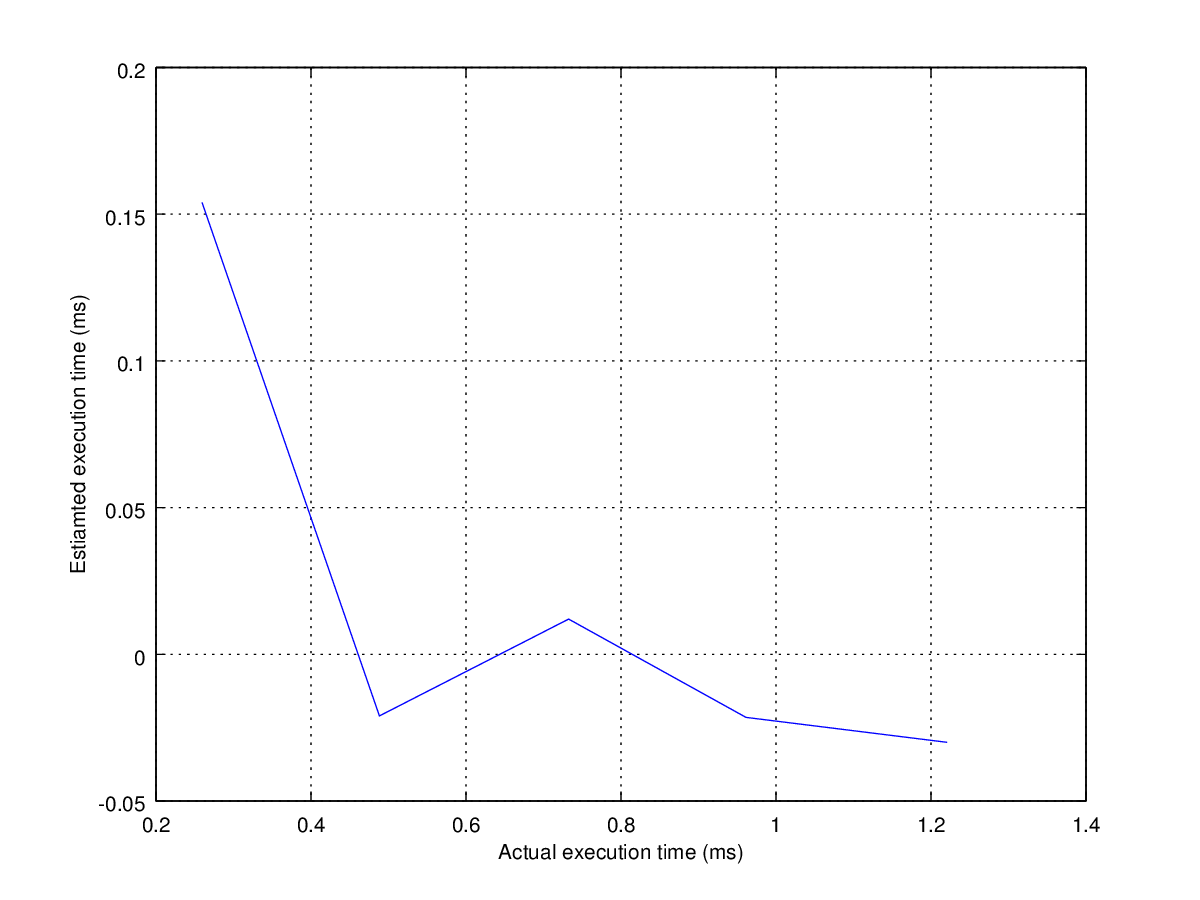
\includegraphics[width=\linewidth]{fig/lowtaest.png}
	\subcaption{Estimated execution time $\hat{t}_A$}
	\end{subfigure}
	\begin{subfigure}{0.45\linewidth}
	\center
	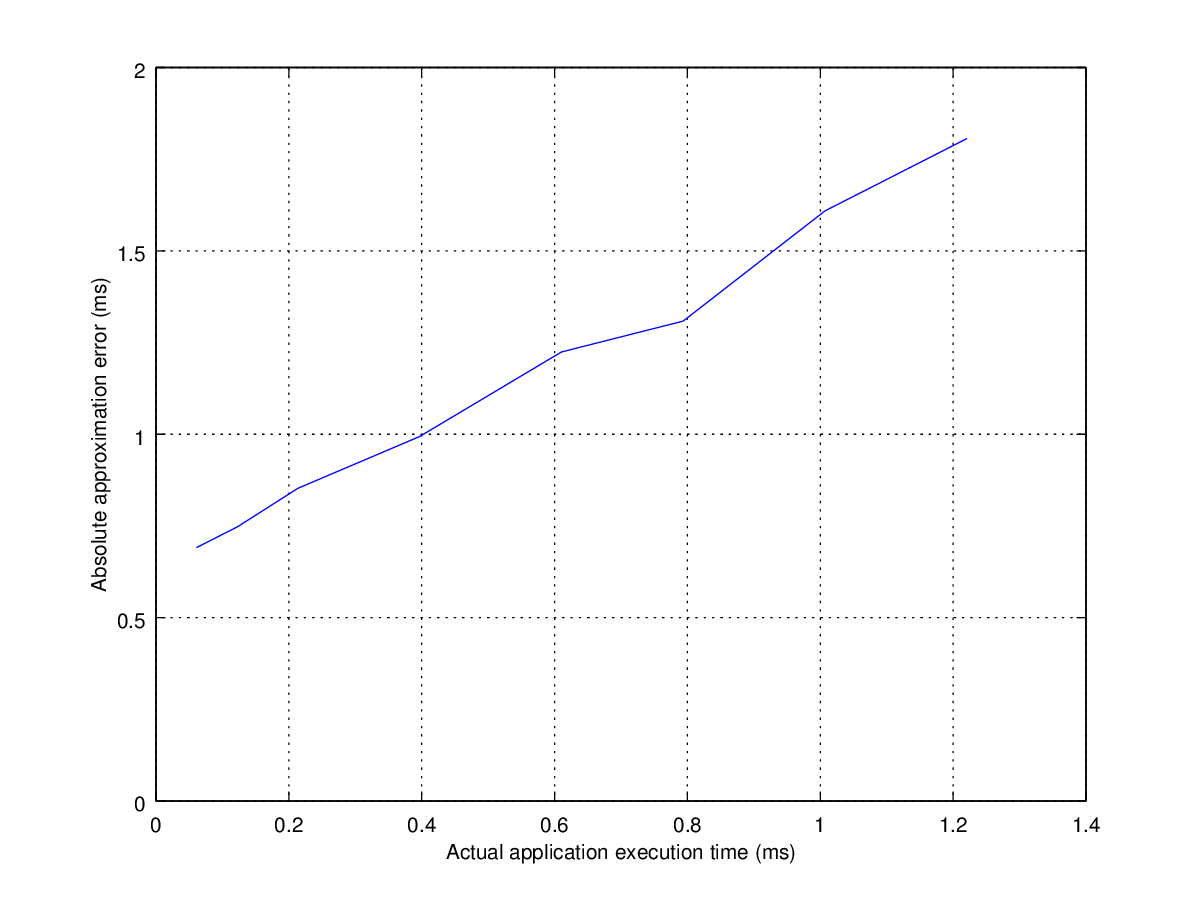
\includegraphics[width=\linewidth]{fig/lowabstaerr.png}
	\subcaption{Absolute approximation error $\epsilon$}
	\end{subfigure}
	\begin{subfigure}{0.45\linewidth}
	\center
	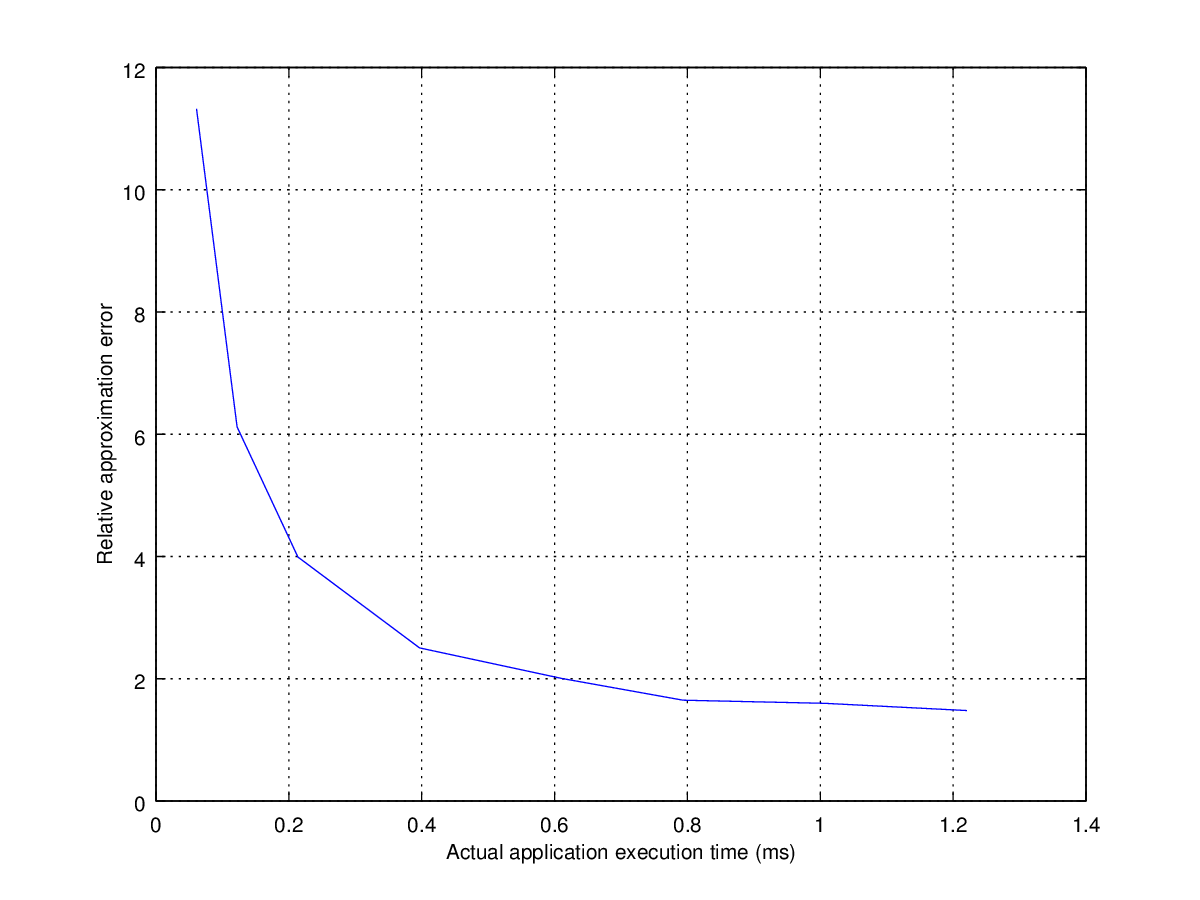
\includegraphics[width=\linewidth]{fig/lowrtvtaerr.png}
	\subcaption{Relative approximation error $\mu$}
	\end{subfigure}
	\caption{Estimation for low $t_A$($<1.5$ms) on CC2538}
	\label{Fig: Estimation for low tA}
\end{figure}

The result in \Cref{Fig: Estimation for low tA} indicates that the estimation totally failed at low $t_A$ such that even negative values are estimated. We consider this is caused by the fact that at such level $t_A$ is negligible and is dominated by noise. $\epsilon$ increases nearly linearly with $t_A$, whilst $\mu$ indicates that the estimation does not make much sense at this level of $t_A$.

\subsubsection{Medium Execution Time}

For $t_A$ with medium values ($t_A \in[1.5, 100)$ ms), the results are shown in \Cref{Fig: Estimation for medium tA}.

\begin{figure}[ht!]
	\center
	\begin{subfigure}{0.8\linewidth}
	\center
	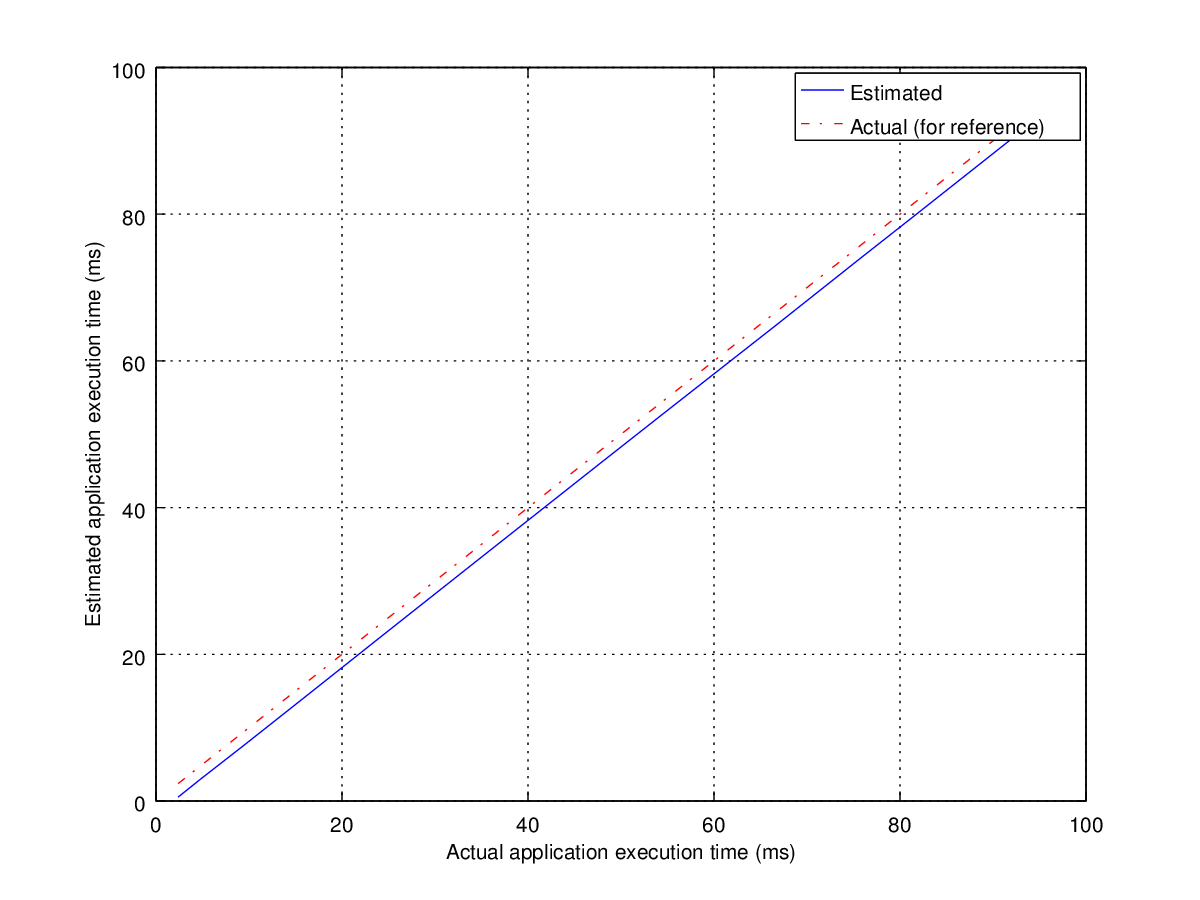
\includegraphics[width=\linewidth]{fig/midtaest.png}
	\subcaption{Estimated execution time $\hat{t}_A$}
	\end{subfigure}
	\begin{subfigure}{0.45\linewidth}
	\center
	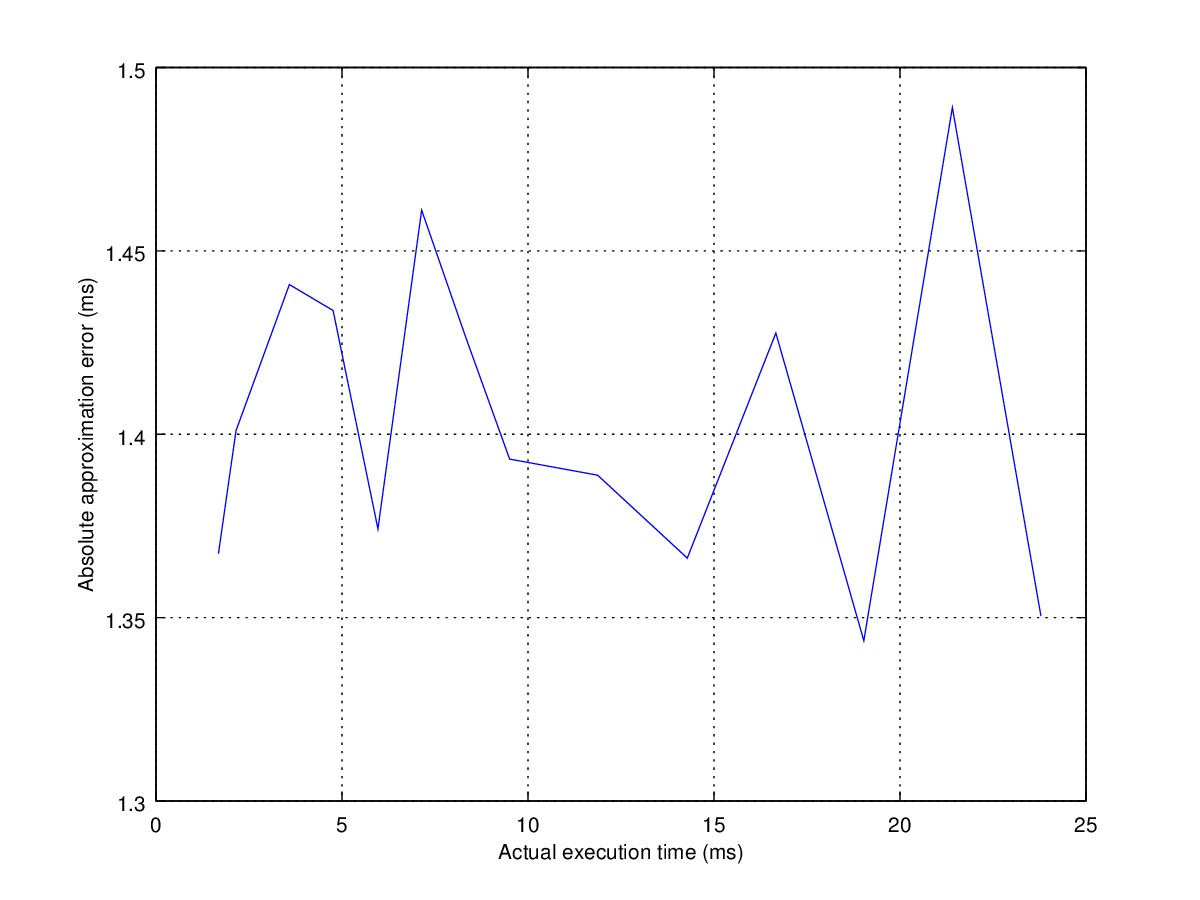
\includegraphics[width=\linewidth]{fig/midabstaerr.png}
	\subcaption{Absolute approximation error $\epsilon$}
	\end{subfigure}
	\begin{subfigure}{0.45\linewidth}
	\center
	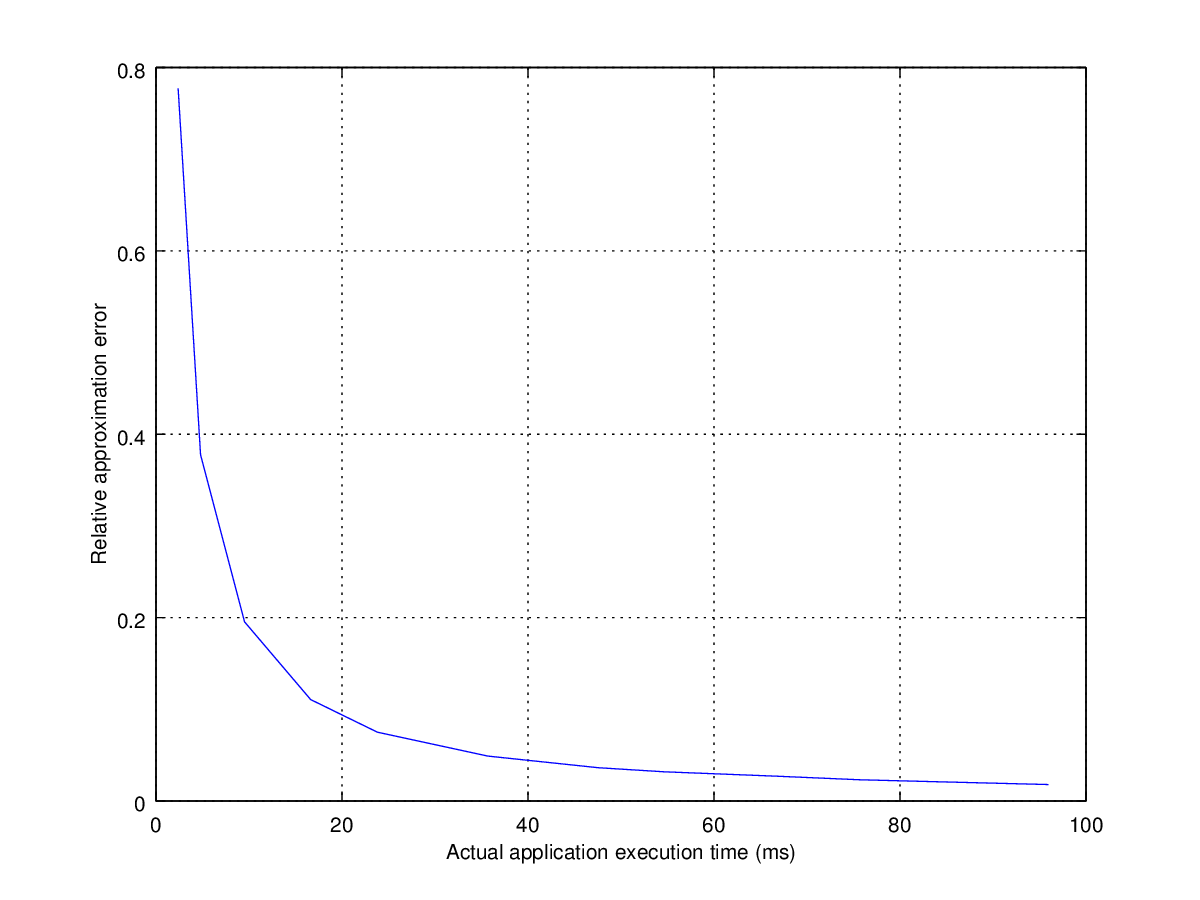
\includegraphics[width=\linewidth]{fig/midrtvtaerr.png}
	\subcaption{Relative approximation error $\mu$}
	\end{subfigure}
	\caption{Estimation for medium $t_A$($[1.5,100)$ ms) on CC2538}
	\label{Fig: Estimation for medium tA}
\end{figure}

$\hat{t}_A$ increase nearly linearly with $t_A$ in \Cref{Fig: Estimation for medium tA}. However, we realised that our estimations are strictly beneath the actual value. $\epsilon$ appears to be random with medium $t_A$,  ranging between $[1.34, 1.49]$ ms.  The sample mean and standard deviation for $\epsilon$ are $1.405$ and $0.043$ ms respectively in these experiments. Due to the narrow range of $\epsilon$, $\mu$ decreases inverse proportionally as $t_A$ increases.

Applying least squares fitting, we have an estimation of medium $t_A$:
\begin{equation} \label{Eq: midta}
	t_A = 1.412 + 0.999\hat{t}_A 
\end{equation}

with $R^2=1.000$, $F=3.45 * 10^5$ ($F_{0.05} = 4.7472$) which suggests that $\hat{t}_A$ is linearly related to $t_A$. 

Theoretically, we hope $t_A = \hat{t}_A$. The result of \Cref{Eq: midta} implies that there exists a systematic bias in our estimation such that we underestimated $t_A$ by roughly $1.4$ ms. On the other hand, the slope of $0.999$ also suggests that the differential estimation is relatively reliable such that its error is roughly less than $0.025$ ms within medium $t_A$.

\subsubsection{High Execution Time}

Further increasing $t_A$, we have the results for high $t_A$ ($\geq 25$ ms) shown in \Cref{Fig: Estimation for high tA}.

\begin{figure}[ht!]
	\center
	\begin{subfigure}{0.8\linewidth}
	\center
	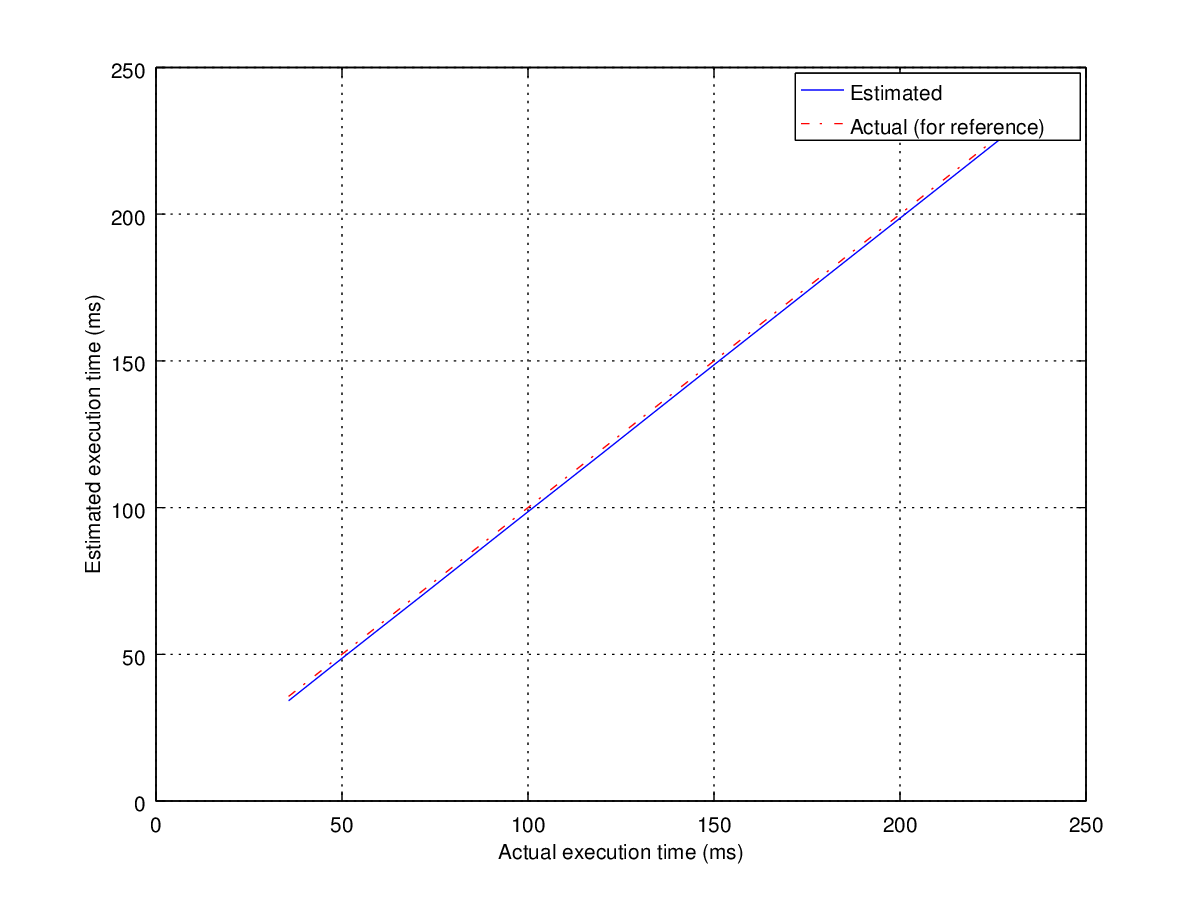
\includegraphics[width=\linewidth]{fig/hightaest.png}
	\subcaption{Estimated execution time $\hat{t}_A$}
	\end{subfigure}
	\begin{subfigure}{0.45\linewidth}
	\center
	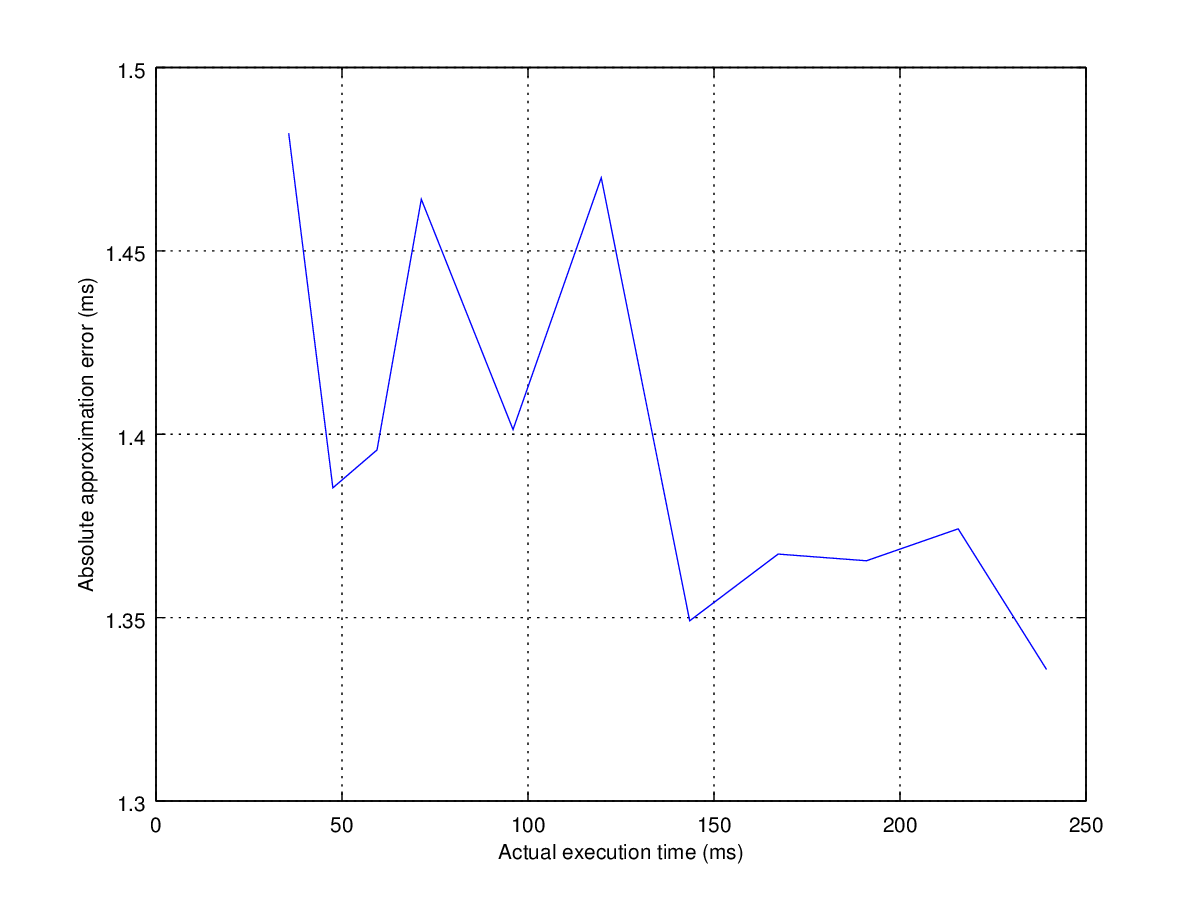
\includegraphics[width=\linewidth]{fig/highabstaerr.png}
	\subcaption{Absolute approximation error $\epsilon$}
	\end{subfigure}
	\begin{subfigure}{0.45\linewidth}
	\center
	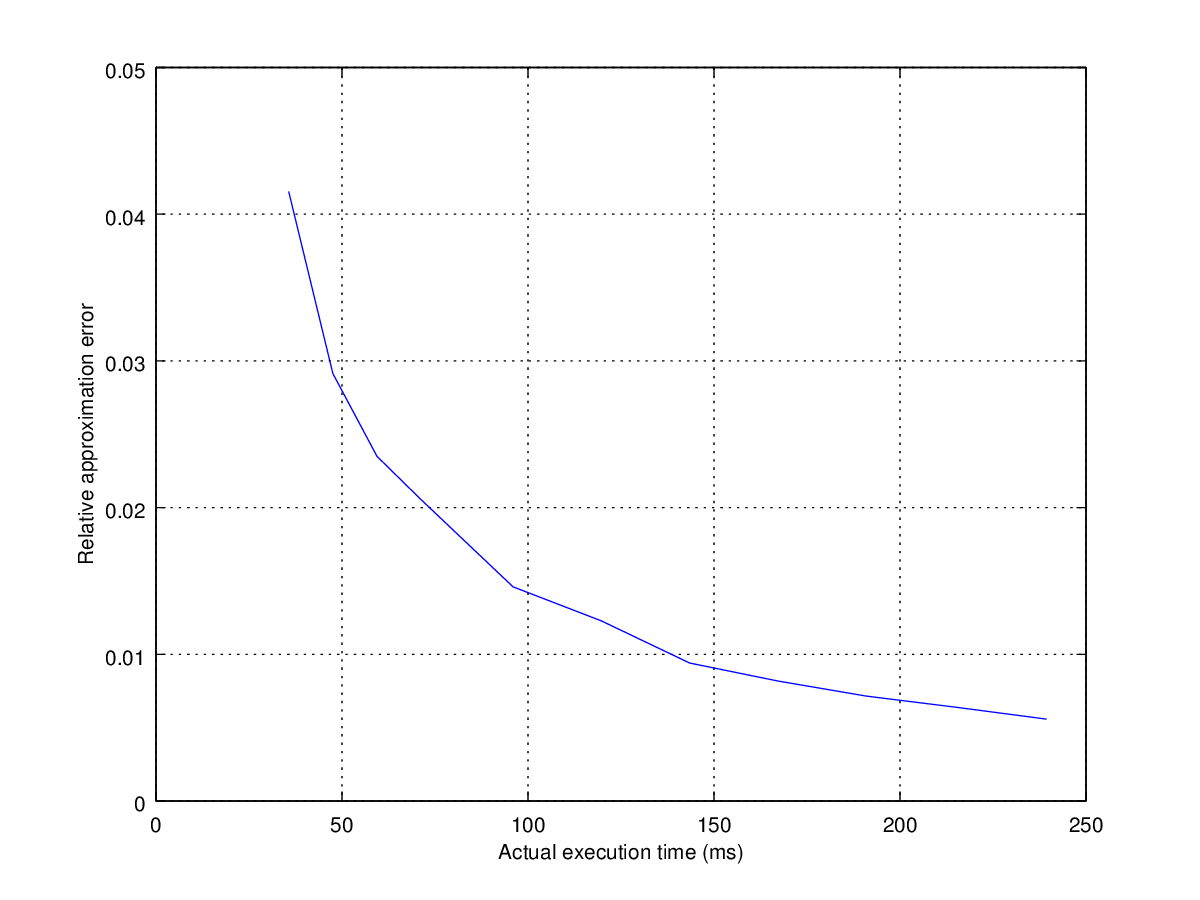
\includegraphics[width=\linewidth]{fig/highrtvtaerr.png}
	\subcaption{Relative approximation error $\mu$}
	\end{subfigure}
	\caption{Estimation for high $t_A$($\geq 100$ ms) on CC2538}
	\label{Fig: Estimation for high tA}
\end{figure}

The result for high $t_A$ is similar to medium $t_A$ such that $\hat{t}_A$ is almost overlapped to $t_A$. The least square estimation of $t_A$ in this group is:
\begin{equation} \label{Eq: hita}
	t_A = 1.459 + 1.000\hat{t}_A
\end{equation}
with $R^2 = 1.000$, $F=3.21 * 10^{7}$ ($F_{0.05} = 5.1174$), which also implies that $t_A$ and $\hat{t}_A$ are linearly related.

$\epsilon$ and $\mu$ are also similar to their counterpart of medium $t_A$ that $\epsilon$ seems to be random in a small range whilst $\mu$ appears to be inverse proportionally decreasing.

Further more, we realised that the regression model of \Cref{Eq: midta} and \Cref{Eq: hita} are similar. We applied the regression coefficient equality test proposed by \cite{CoeEqTest}. The test returns $F=0.010$ ($F_{0.05} = 3.47$), indicates that \Cref{Eq: midta} and \Cref{Eq: hita} are likely to be the same regression model.

\subsubsection{Summary}

In conclusion, our estimation for CC2538 is unreliable when $t_A < 1.5$ ms. For $t_A \geq 1.5$ ms, the estimation is relatively reliable and relative accuracy increases as $t_A$ increases.

We further analysis the error in \Cref{ta error}.

\subsection{Errors} \label{ta error}

The absolute approximation error $\epsilon$ is defined to be signedness. We define the signed approximation error :
\begin{equation} \label{Eq: e}
e = t_A - \hat{t}_A
\end{equation}

We show the overall signed approximation error among all $t_A$ in \Cref{Fig: Overall approximation error}.

\begin{figure}[ht!]
	\center
	\begin{subfigure}{0.45\linewidth}
		\center
		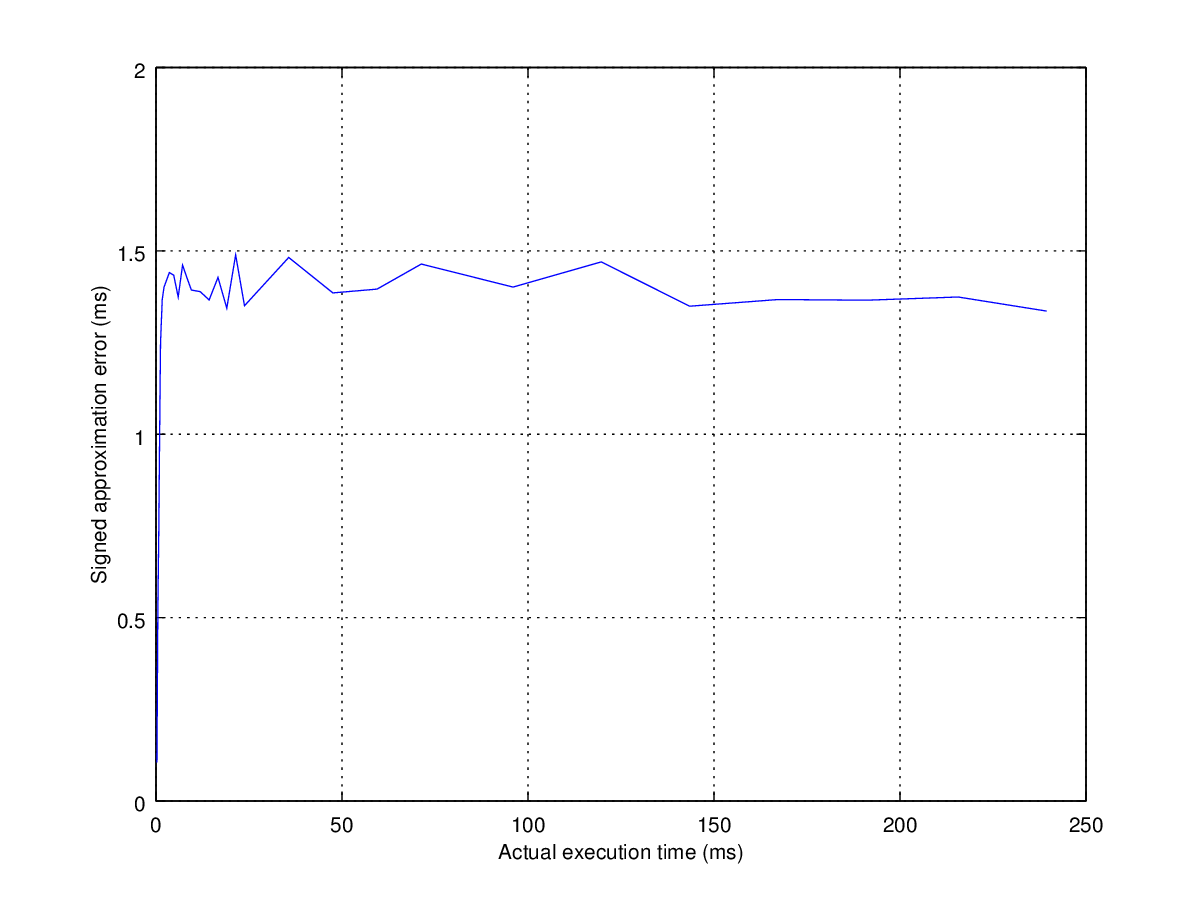
\includegraphics[width=1\linewidth]{fig/esterr.png}
		\subcaption{Signed approximation error ($e$)}
	\end{subfigure}
	\begin{subfigure}{0.45\linewidth}
		\center
		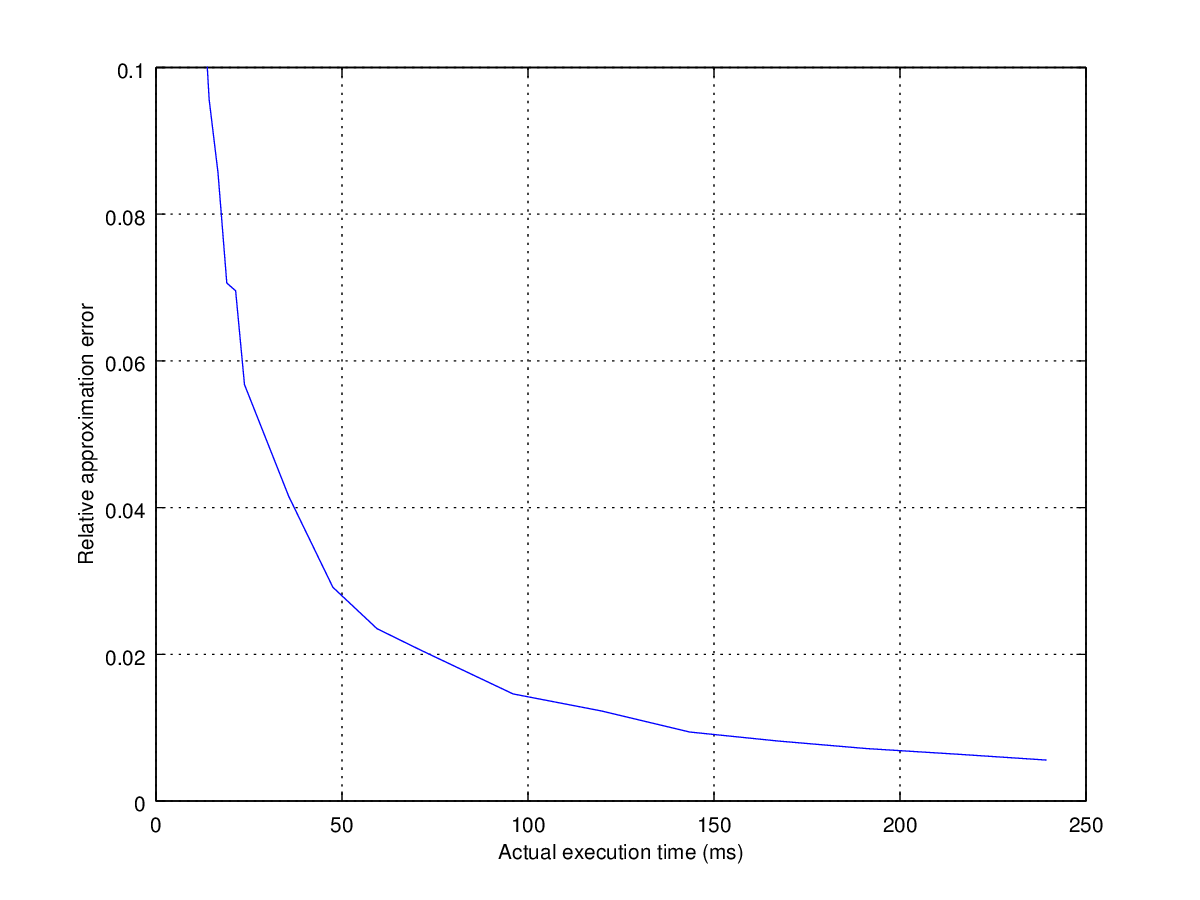
\includegraphics[width=\linewidth]{fig/rtvesterr.png}
		\subcaption{Relative estimation error ($\mu$), for $< 0.1$}
	\end{subfigure}
	\caption{Overall approximation error}
	\label{Fig: Overall approximation error}
\end{figure}

The result suggests that $e$ dramatically increases at low $t_A$ but quickly converges to [1.34, 1.49] at higher $t_A$. For the converged $e$, (i.e. when $t_A > 1.5$ ms), the sample mean and standard deviation of $e$ are $1.402$ ms and $0.046$ ms respectively. Using Shapiro-Wilk nomality test on $e$, the result was $W = 0.934$ ($W_{0.05} = 0.918$), suggesting that $e$ is likely to be normally distributed.

From a practical aspect, it would be reasonable to simply approximate the negligible low $t_A$ as $0$ ms. Observing \Cref{Fig: Estimation for low tA}, we suggest to discard the estimations when $\hat{t}_A < 0.1$ as different $t_A$ may confusingly mapped to same $\hat{t}_A$. In another word,the low $t_A$ would be unmeasureable from the captured traffic by this method.

Considering the fact that the sample mean of $e$ is much greater than its standard deviation, we suppose it is dominated by a systematic error. The potential factors of the error we have considered include:
\begin{itemize}
	\item Implicit affection of application code.
	\item Error in estimation of $t_P$.
\end{itemize}

Therefore we conducted comparison experiments to study the impact to $e$ of these factors, showed in the following context.

\subsubsection{Implicit affection of application code} \label{Affection of application code}

As a comparison, we replace the random number generator by Contiki software AES encryption and then measured the error as we have done on \Cref{apptime}. The result is shown in \Cref{Fig: Overall estimation error for AES replacement}.

\begin{figure}[ht!]
	\center
	\begin{subfigure}{0.45\linewidth}
		\center
		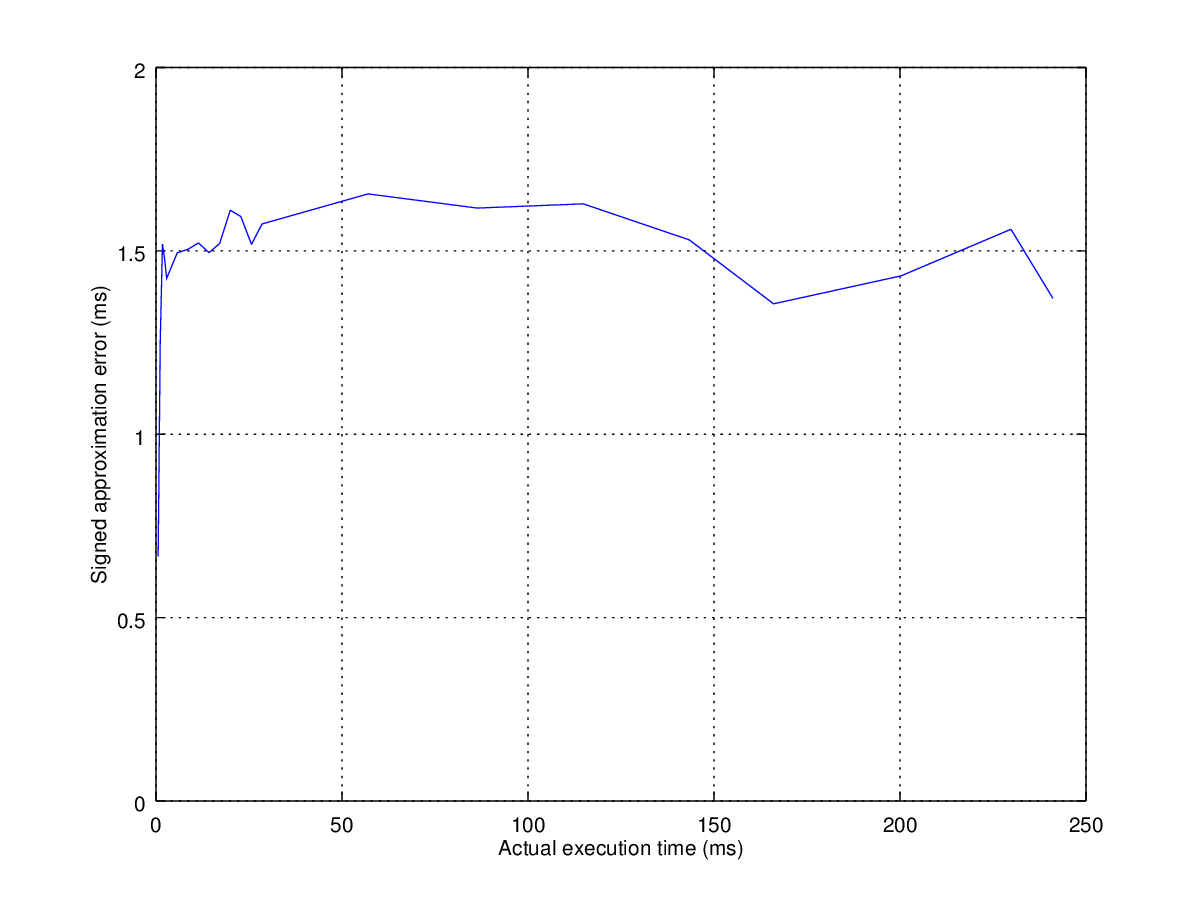
\includegraphics[width=1\linewidth]{fig/esterraes.png}
		\subcaption{Signed approximation error ($e$)}
	\end{subfigure}
	\begin{subfigure}{0.45\linewidth}
		\center
		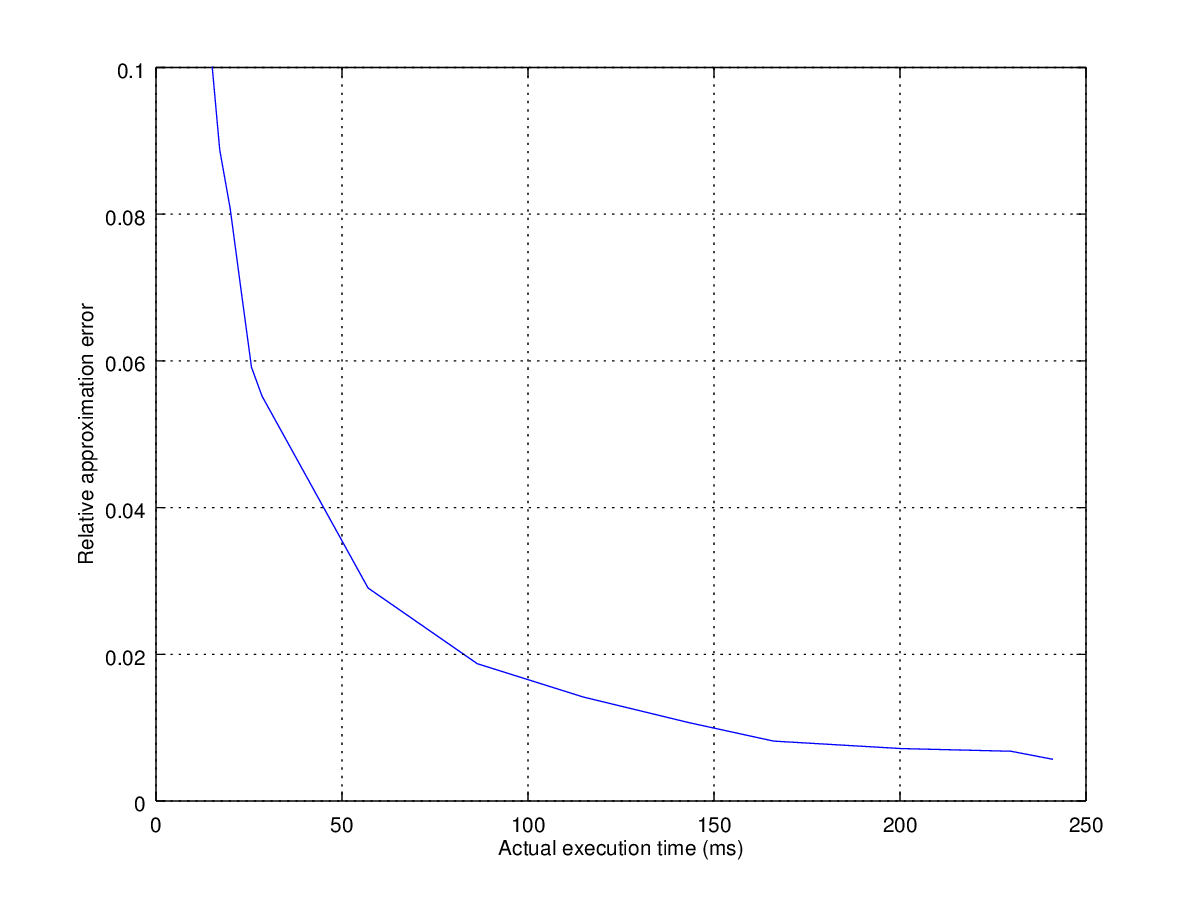
\includegraphics[width=\linewidth]{fig/rtvesterraes.png}
		\subcaption{Relative estimation error ($\mu$), for $< 0.1$}
	\end{subfigure}
	\caption{Overall approximation error for AES replacement}
	\label{Fig: Overall estimation error for AES replacement}
\end{figure}

We denote $e_{R}$ and $e_{A}$ to be the singed approximation errors in the original application with random number call (the application showed in \Cref{apptime}) and its AES encryption replacement. Intuitively,  \Cref{Fig: Overall estimation error for AES replacement} showed that $e_{A}$ has some similar characteristics as of $e_{R}$:
\begin{itemize}
	\item They both dramatically increases at low $t_A$, then converges into a small range for medium and high $t_A$.
	\item The relative approximation error $\mu$ decreases nearly inverse proportionally, reaching $<0.1$ at $25$ ms.
\end{itemize}

The converged sample mean and standard deviation for $e_A$ are $1.520$ ms and $0.082$ ms respectively. Again using Shapiro-Wilk normality test, we have $W=0.962$ ($W_{0.05} = 0.904$), indicating $e_{A}$ is also likely to be normally distributed. We summarise some basic statistical features of $e_R$ and $e_A$ in \Cref{Tbl: Statistical features of eR and eA}.

\begin{table}[ht!]
	\center
	\begin{tabular}{|c|c|c|}
	\hline
	      & Sample Mean (ms) & Sample Standard Deviation (ms) \\ \hline
	$e_{RND}$ & 1.402            & 0.046                          \\ \hline
	$e_{AES}$ & 1.520            & 0.082                          \\ \hline
	\end{tabular}
	\caption{Statistical features of $e_{RND}$ and $e_{AES}$}
	\label{Tbl: Statistical features of eR and eA}
\end{table}

Two sample t-test on $e_R$ and $e_A$ returned $p=2.32 * 10^{-7}$, indicating their mean might be different; thus replacing random number generator to AES may have impacted $e$.

The reason of why such replacement affected $e$ is so far unclear. Theoretically, since there is no data dependency between the timed code and other parts of the code, they are normally considered independent. On the other hand, different sequence of code execution, i.e. different number of loops, does not affect such error, suggesting it is might be caused by a static change of  system state that we are not aware of. We leave this as an open question in this report. However in practice, we would argue that such error can be mitigated as $t_A$ increases, as depicted by the relative approximation errors in \Cref{Fig: Overall approximation error} and \Cref{Fig: Overall estimation error for AES replacement}. We also expect the difference of this error among applications to be minor as there is no known data dependency.

\subsubsection{Error in estimation of protocol suite processing time}

Substituting \Cref{Eq: t_A} and \Cref{Eq: hattA} into \Cref{Eq: e}, we have:

\begin{equation}\label{Eq: tP error}
	\begin{aligned}
		e &= t_A - \hat{t}_A = (t_R - t_P) - (t_R - \hat{t}_P) = \hat{t}_P - t_P\\
		t_P &= \hat{t}_P - e
	\end{aligned}
\end{equation}

\Cref{Eq: tP error} implies that $e$ can be also viewed as the residual of the error of $\hat{t}_P$. However, our experiments in \Cref{Affection of application code} suggests that $e$ has dependency to the application code. \Cref{Eq: CC2538tP} does not captured this as $\hat{t}_P$ is solely decided by $|Req|$ and $|Res|$. 

We therefore re-estimated the impact of $|Req|$ and $|Res|$ to $\hat{t}_P$ for the code of \Cref{apptime} by:
\begin{equation}
	t_P = t_R - t_A
\end{equation}
where $t_A$ is adjusted to $4.9$ ms and $24.7$ ms respectively. The result is shown in \Cref{Fig: e by len}.

\begin{figure}[ht!]
	\center
	\begin{subfigure}{0.45\linewidth}
		\center
		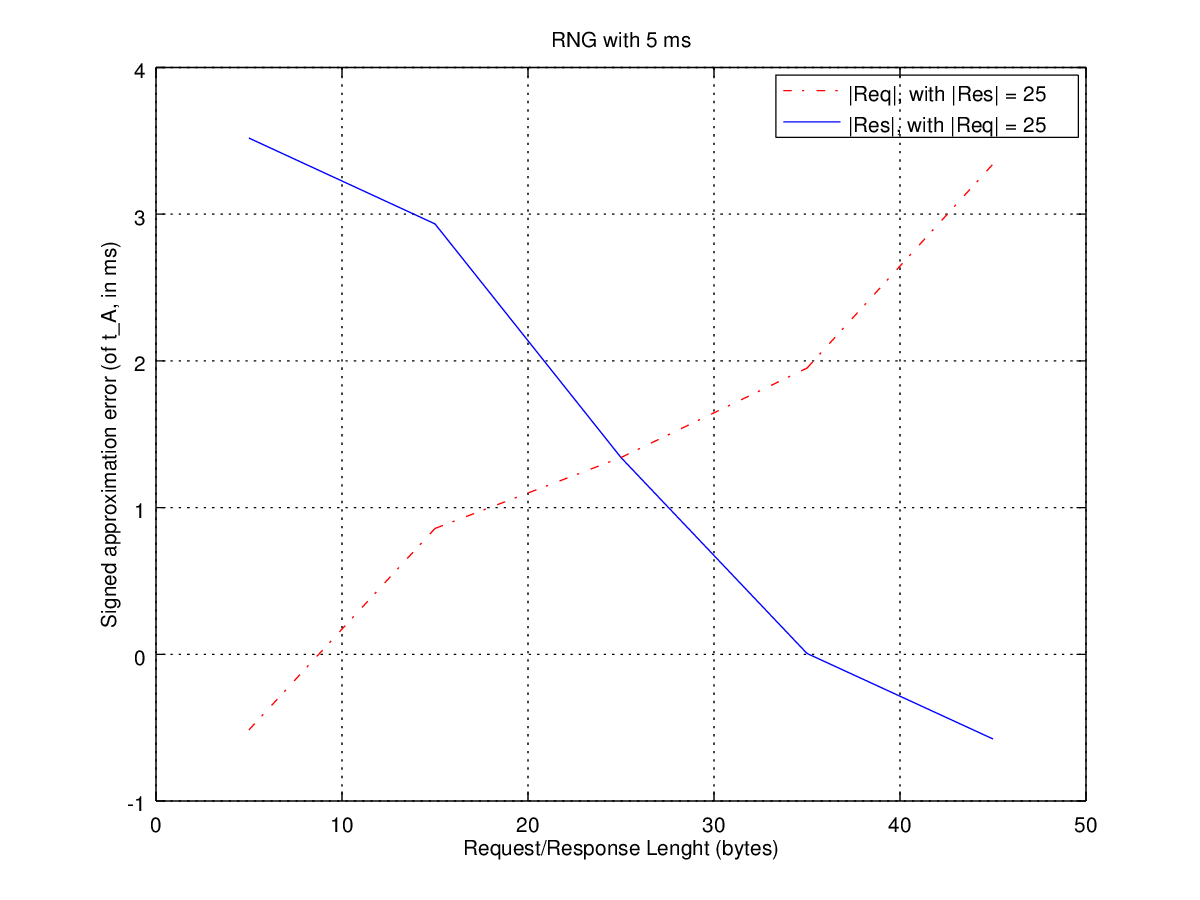
\includegraphics[width=\linewidth]{fig/errwithlen5ms.png}
	\end{subfigure}
	\begin{subfigure}{0.45\linewidth}
		\center
		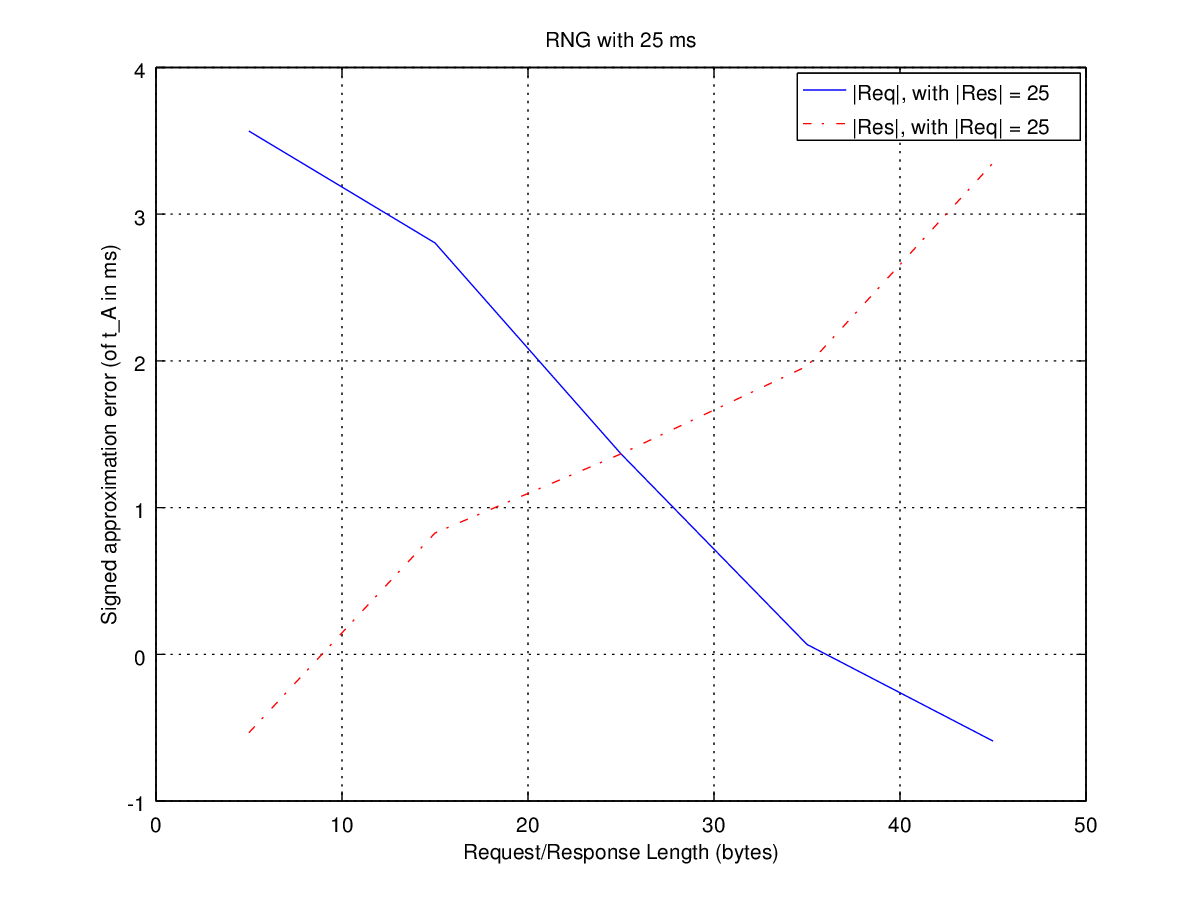
\includegraphics[width=\linewidth]{fig/errwithlen25ms.png}
	\end{subfigure}
	\caption{Affection on $e$ by $|Req|$ and $|Res|$, with Contiki RNG}
	\label{Fig: e by len}
\end{figure}

The result suggests that:
\begin{itemize}
	\item Even with different application code, $e$ still seems to be multi linearly related to both $|Rea|$ and $|Res|$.
	\item Change of $t_A$ does not seem to affect $e$.
\end{itemize}

Apply multiple linear regression on the results for each $t_A$, we have two regression models:
\begin{equation}
	\hat{e} = 2.007 - 0.111|Req| + 0.088|Res|
\end{equation}
with $R^2 = 0.971$ for $t_A = 4.9$, and

\begin{equation}
	\hat{e} = 1.962 - 0.111|Req| + 0.089|Res|
\end{equation}
with $R^2 = 0.978$ for $t_A = 24.7$.

Again using the coefficient equality test on both regression models, the test reports no statistical significance on the coefficients of the regression models. Therefore we re-estimate $e$ using the full data. The estimation is:
\begin{equation} \label{hate}
	\hat{e} = 1.984 - 0.111|Req| + 0.089|Res|
\end{equation}
%Show Fstat!!!!! CONTINUE HERE
with $R^2 = 0.975$.

Recall the fact that the length of packets are constrained by 802.15.4 MTU and thus $|Req| \in [0,47]$ and $|Res| \in [0,46]$, we have $\hat{e} \in [-3.233,6.078]$ ms. Although $\hat{e}$ might be hard to predict as it is related to specific application code, in our experiment, $e$ is in a relatively small range. In practice, we would expect that such level of error is tolerable, especially when estimating application code with longer execution time.

\subsection{Differential Analysis}

Sometimes the difference in execution time may also be an interested target to an adversary. 

Denote $\Delta t_A$ to be the difference in application code execution time of two Sessions of the same device, we have:
\begin{equation}\label{Eq: delta t}
	\begin{aligned}
		\Delta t_A &= t_A - t'_A \\
			&= (t_R - t_P) - (t'_R - t'_P) \\
			&= t_R - t'_R - (t_P - t'_P) \\
			&= t_R - t'_R - [(\hat{t}_P - e) - (\hat{t'}_P - e')] \\
			&= t_R - t'_R - \hat{t}_P - \hat{t'}_P - (e - e')
	\end{aligned}
\end{equation}
 
Notice that in \Cref{Eq: delta t}, $t_R$ and $t'_R$ are directly observable from the captured traffic. $\hat{t}_P$ and $\hat{t'}_P$ can solely calculated by $|Req|$ and $|Res|$ which are also directly observable in the packets. This left only $(e-e')$ the uncertainty in \Cref{Eq: delta t}.

On the other hand,  based on the results shown in \Cref{Tbl: Statistical features of eR and eA}, we suppose  the variance of $e$ might be negligible in practice and therefore so is $(e - e')$. In this case, we suggest to approximate \Cref{Eq: delta t} as:
\begin{equation}
	\Delta t \approx t_R - t'_R - \hat{t}_P - \hat{t'}_P = \hat{t}_A - \hat{t'}_A
\end{equation}

However, we consider $(e - e')$ difficult to further quantified, as its value can be affected by the application code (as shown in \Cref{Affection of application code} ) which can hardly be quantified without knowing exactly how it affects the execution time.

\subsection{Execution time of CoAP Implementation}

CoAP, described in \Cref{Subsec: CoAP}, is an interesting target in real world WSN applications. Although the secure version, CoAPs, has not been implemented in Contiki release-3.0 yet, the execution time of CoAP can be considered as a reference to CoAPs, as CoAP directly maps to the application code in \Cref{Fig: A Session with DTLS} during a CoAPs session.

We measured the execution time of CoAP on CC2538 by the coaptime application,  derived from the er-example-server application in Contiki examples. A timing module is also added to the CoAP implementation. 

The available resources on coaptime are described in \Cref{Tbl: Resources on coaptime}.

\begin{table}[ht!]
	\center
	\begin{tabular}{|c|c|l|}
		\hline
		Resource & Method & \multicolumn{1}{c|}{Description}                          \\ \hline
		toggle   & POST   & Toggle the red LED.                                       \\ \hline
		sensors  & GET    & Read all sensors on the board (VDD, temperature and ALS). \\ \hline
		als      & GET    & Read Ambient Light Sensor, ALS.                           \\ \hline
		tmp      & GET    & Read temperature sensor.                                  \\ \hline
		vdd      & GET    & Read voltage sensor.                                      \\ \hline
		hello    & GET    & Return a string of "Hello world!".                        \\ \hline
		timing   & GET    & Return the last CoAP request processing time.             \\ \hline
	\end{tabular}
	\caption{Resources on coaptime}
	\label{Tbl: Resources on coaptime}
\end{table}

The processing time of each Coap requests are summarised in \Cref{Tbl: Coap requests processing time of coaptime}.

\begin{table}
	\center
	\begin{tabular}{|c|c|c|}
		\hline
		Resource & Processing time (Clock Ticks) & Processing time (ms) \\ \hline
		toggle   & 9.70                          & 0.30                 \\ \hline
		sensors  & 99.75                         & 3.04                 \\ \hline
		als      & 85.16                         & 2.60                 \\ \hline
		tmp      & 18.67                         & 0.57                 \\ \hline
		vdd      & 16.77                         & 0.51                 \\ \hline
		hello    & 6.30                          & 0.19                 \\ \hline
	\end{tabular}
	\caption{Coap requests processing time of coaptime, on CC2538}
	\label{Tbl: Coap requests processing time of coaptime}
\end{table}

The results in \Cref{Tbl: Coap requests processing time of coaptime} suggests that the processing time of sensors and als had fell into the medium $t_A$ category ($[1.5, 25)$ ms), which are potentially distinguishable by timing information when used in CoAPs.

The source code of our coaptime application and the timed CoAP implementation are available at: \\
\url{https://github.com/Salties/MyRepository/tree/master/experiments/coaptime}\\
and \\
\url{https://github.com/Salties/MyRepository/tree/master/er-coap} \\
respectively.

%DTLS has potentially the best interoperability as it is an variation of the widely used TLS in Internet. However, its design might not fit into the nature of WSN for practical reasons.
%
%\section{Implementation Issues}
%The most practical implementation we found on Contiki OS so far is tinydtls.
%
%tinydtls\cite{tinydtls} currently supports two ciphersuites, namely TLS\_PSK\_WITH\_AES\_128\_CCM\_8 and TLS\_ECDHE\_ECDSA\_WITH\_AES\_128\_CCM\_8. 
%
%However, we encountered several difficulties when trying to set up an encrypted network using tinydtls.
%
%\begin{description}
%\item[Low Computational Power] \hfill \\
%Curve computation requires relatively a large amount of computational power. Even using a relatively powerful platform (CC2538), it still takes minutes to complete a DTLS handshake with
%TLS\_ECDHE\_ECDSA\_WITH\_AES\_128\_CCM\_8.
%
%\item[Low Bandwidth] \hfill \\
%The 6LowPAN standard specifies that the minimum MTU is 127 bytes whilst 67 (87 with LLSEC) bytes are occupied by protocol headers until UDP, which leaves 60 (40 with LLSEC) bytes available for UDP layer payload. This value has been exceeded by several handshake packets even with pre-shared keys. Doing key exchange or even using longer keys only makes this problem worse. Some attempts have been made to solve this issue, e.g. CoDTLS\cite{CoDTLS}\footnote{This draft has been abandoned for some reason we do not know.}. As a result, DTLS is only available on those devices support extra frame length than 6LowPAN requirements.
%
%\item[Code Size] \hfill \\
%The tinydtls fails to fit into some devices, e.g. skymote, as its size of code is too large.
%\end{description}
%
%Therefore although TLS\_PSK\_WITH\_AES\_128\_CCM\_8 is less flexible (and probably less secure) as it uses a pre-shared master secret, it is still considered to be a relatively practical security measure as it requires less resources.
%
%\section{No Multicast Support}
%Some application protocols, such as CoAP, utilises the multicast feature of 6LowPAN whilst TLS is a protocol designated for securing communications between two parties, so is DTLS. To  our knowledge, DTLS does not make any attempt to support multicasting.
%
%\section{Overloading DTLS with LLSEC}
%Adopting both security measures at the same time is possible as they are implemented at different layers. However, it is questionable whether this will bring more security, as both {\it noncoresec} and TLS\_PSK\_WITH\_AES\_128\_CCM\_8 are using 128 bit AES with CCM mode as their cryptographic primitive.
